 \subsection{Mixtures of Gaussians}

Mixtures of Gaussian or the Gaussian Mixture Model (GMM) is a method of clustering data that's able to disentangle ambiguous samples by considering a sample's probability of belonging to a class, known as a soft assignment. 

Initially, K Gaussian functions are randomly generated corresponding to K clusters. If a dataset has low dimensionality, by taking a histogram of its values the Gasussian's initial conditions can be approximated, as in Figure \ref{fig:mixture}. By superpositioning all of the Gaussians a sample's complete probabilistic model is created, i.e. a model for \emph{all} clusters. 

\begin{figure}[H]
	\centering
	\begin{subfigure}[b]{0.5\linewidth}
            \centering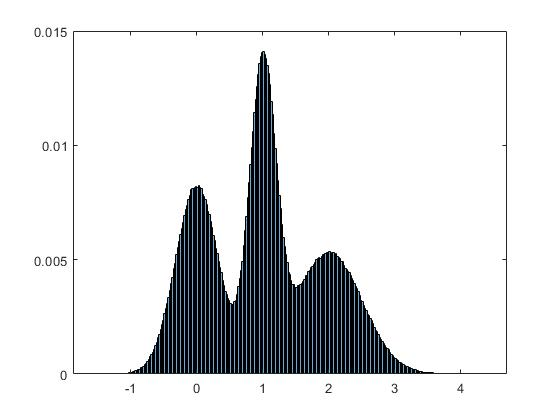
\includegraphics[width=215pt]{histGauss}
      		\caption{Normalized Histogram of 1D samples.}
		\label{fig:histGauss}
    	\end{subfigure}%
    	\begin{subfigure}[b]{0.5\linewidth}
      		\centering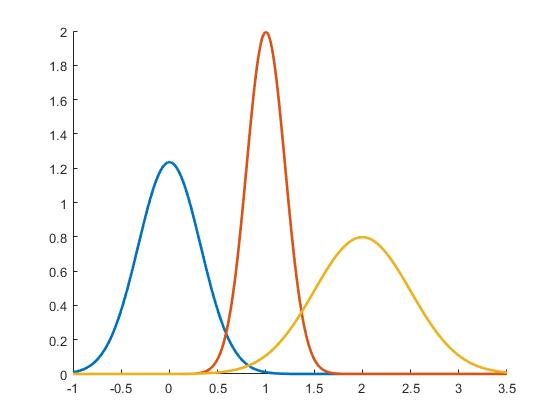
\includegraphics[width=215pt]{hist_gauss_curve}
      		\caption{Gaussians derived from 1D histogram. }
       		\label{fig:histCurve}
		\end{subfigure}
		\caption{Formulation of Mixture of Gaussians.}
    	\label{fig:mixture}
\end{figure}

With each iteration of the GMM algorithm the parameters of the model's component Gaussians are tuned according to the covariance (\ref{eq:cov}) between samples in each cluster. $X$ and $Y$ are the variables being compared, $\overline X$ and $\overline Y$ are variable means and $n$ is the number of samples. For a multidimensional dataset this results in a covariance matrix $\bm{\Sigma_k}$ for each Gaussian, furthermore a multidimensional Gaussian requires also a mean vector $\bm{\mu_k}$ as opposed to scalar. 

\begin{equation}
Cov(X, Y) = \frac{\Sigma(X_i-\overline X)(Y_j-\overline Y)}{n}
\label{eq:cov}
\end{equation}



The algorithm seeks the highest covariance possible in each of its clusters. It is by considering the covariance of samples that the GMM is able to best classify ambiguous samples. The higher the covariance (aka correlation) between sample dimensions the more likely it is they belong in the same cluster. This can observed in Figure \ref{fig:mogcov}, the data being clustered is the same as in Figure \ref{fig:clusters} but notice the elliptical shape of the Gaussian cluster distributions as opposed to the spherical shape of K-Means clustering.

\begin{figure}[H]
	\centering
	\centering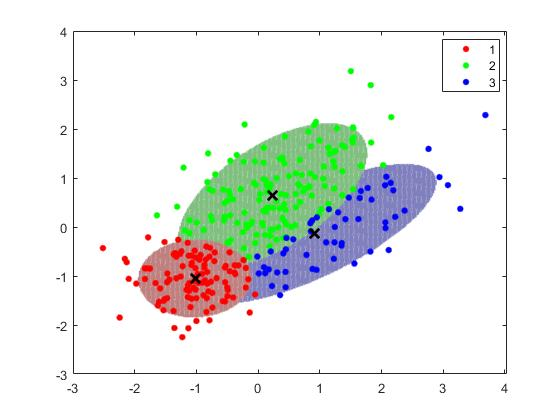
\includegraphics[width=450pt]{mog}
	\caption{Clustering using GMM.}
	\label{fig:mogcov}
\end{figure}
  
Within the complete mixture model the probability a sample belongs in one of them is 100\%. In Figure \ref{fig:histScale} the Gaussians from Figure \ref{fig:histCurve} have been scaled to have the amplitudes $\pi_1 = 0.3$, $\pi_1 = 0.5$ and $\pi_1 = 0.2$. These are weightings that give the mixing ratio of the model and represent a cluster's proportion of the total samples. The more samples a cluster contains the more likely it is a sample belongs to it. The sum of ratios must add to one because the probability a sample belongs to at least one cluster is one, as defined in \ref{eq:gauss_weight1} and \ref{eq:gauss_weight2}.

\begin{equation}
    0\leq \pi_k \leq 1
\label{eq:gauss_weight1}
\end{equation}
\begin{equation}
    \sum_{k=1}^{K}\pi_k = 1
\label{eq:gauss_weight2}
\end{equation}


\begin{figure}[H]
    \centering
    \centering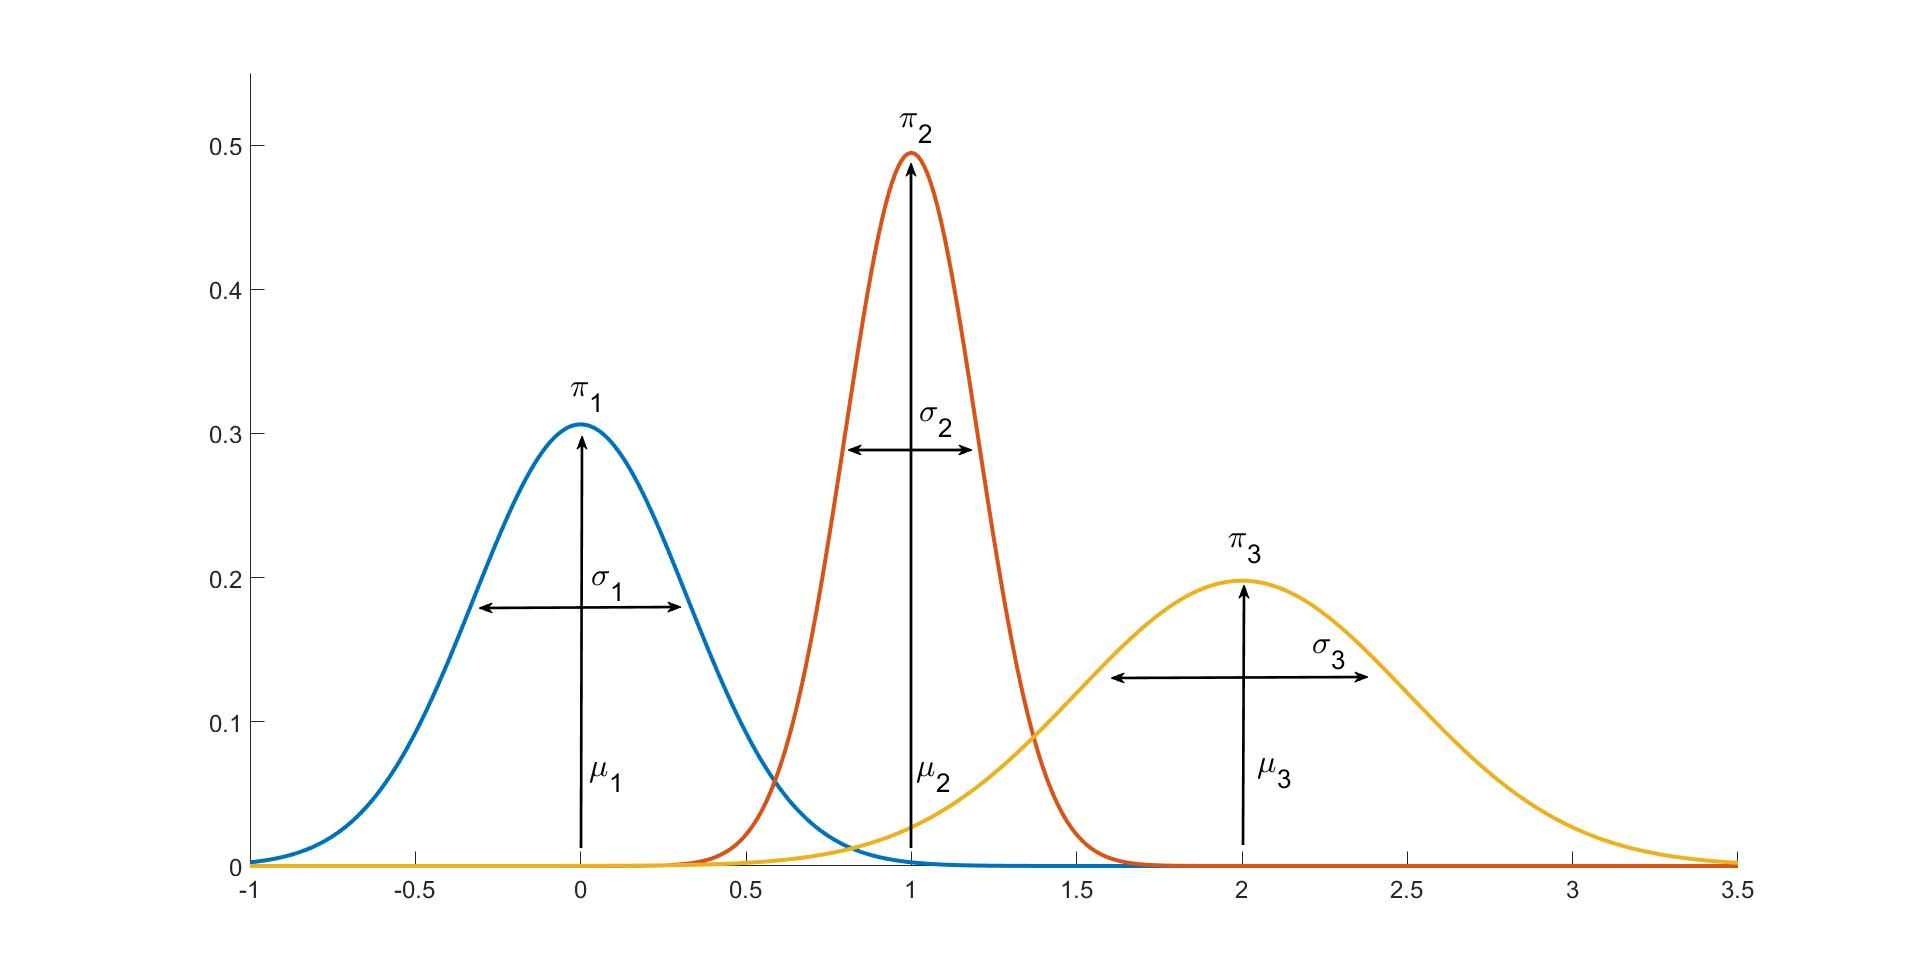
\includegraphics[width=450pt]{gauss_mix_scale}
    \caption{Individual Gaussians with scaled weightings.}
    \label{fig:histScale}
  \end{figure} 

Each Gaussian's three parameters, mean $\mu_k$, ampltidue $\pi_k$ and covariance matrix $\Sigma_k$ are updated following each iteration of the algorithm. This augmentations are performed according to 'Expectation Maximization'.

\subsubsection{Expectation Maximization}

Expectation Maximization (EM) is a method by which to update the parameters of the Gaussian distributions that seeks to maximize a sample's likelihood of belonging to a cluster. 

EM will compute the a sample's proability  of being in a cluster. This value will be used to reestimate the Gaussian proability to better fit the data that is presented by trying to maximizing all sample's probabilities of belonging in a cluster.

The reajustment of the mean of each Gaussian receives weighting from all points proportional to their probability of belonging to that Gaussian's cluster.

The algorithm is comprised of two steps


%% EM STEPS %%
\begin{enumerate}
	\item The \emph{expectation} step estimates the probability the sample $x_i$ belongs to Gaussian cluster $k$.
	\begin{equation}
		z_{ik} = \frac{1}{Z_i}\pi_k\, \mathcal{N}(\bm{x}\,|\,\bm{\mu_k},\bm{\Sigma_k})
	\end{equation}

	\item The \emph{maximization} step aguments the Gaussian parameter values.
	\begin{align*}	
	\tag{eqn1}
	\bm{\mu_k} &= \frac{1}{N_k}\sum_i z_i \bm{x}_i \\
	\tag{eqn2}
	\bm{\Sigma}_k &=  \frac{1}{N_k}\sum_i z_{ik} (\bm{x}_i - \bm{\mu}_k)(\bm{x}_i - \bm{\mu}_k)^T \\
	\tag{eqn3}
	\pi_k &= \frac{N_k}{N}
	\end{align*}
	where \newline
	\centerline{$N_k = \sum_i z_{ik}$}
\end{enumerate}












A cluster indicator $z_i$ exists for every sample, it is the \emph{probability} that the $i$th sample is associated with the $k$th cluster. It is completely specified by the mixture weight $\pi_k$. I.e.

$p(z_i=k) = \pi_k $

If we know that a sample $x_i$ is from cluster $k$ the \emph{likelihood} of seeing it in Gaussian associated with that cluster is

$ p(x_i\, |\, z_i = k, \mu_k, \Sigma_k) = \mathcal{N}(x_i\, |\,\mu_k, \Sigma_k)$ 







for each cluster such that a sample's likelihood of belonging to each cluster is maximized. 






\subsection{Background Subtraction}

This is performed by identifying a background image and then subtracting this image from subsequent frames of video to determine what has changed and hence what is a foreground image.

\subsection{Expectation Maximization}

This is an optimization scheme used to fit a Gaussian Mixture Model. It is an iterative method that faurantees convergence to a local maximum in a search space.